\documentclass[10pt]{article}
\usepackage[margin=0.7in]{geometry}\usepackage[T1]{fontenc}\usepackage{amsmath,amssymb,tikz}
\begin{document}
\section*{UInt64 ordered degree-two guard correspondence}
\textbf{Producer construction; independent source-fidelity review pending.}

The word expression for $B$ is canonical and decodes to
\[
 B=2\big((qs-t)t-(rs)s\big).
\]
The exact word dispatcher selecting \texttt{sameUDouble}, together with literal $B=0$, implies $s\ne0$. Thus its call to the helper cannot select \texttt{b\_zero\_identity}; it reaches the helper's point-doubling arm. This statement does not specify the degree or validity of the eventual doubled payload.

\begin{center}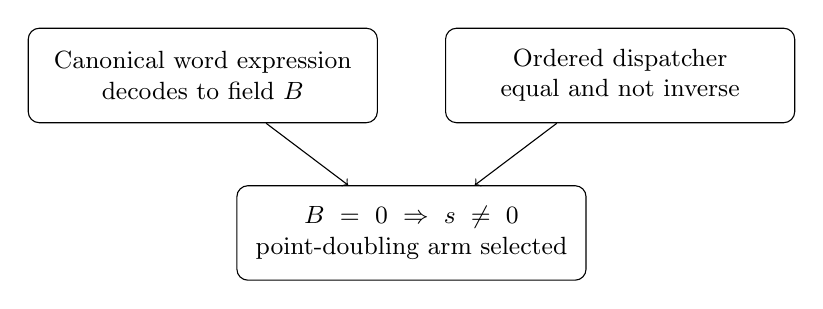
\begin{tikzpicture}[every node/.style={draw,rounded corners,align=center,text width=4.2cm,minimum height=1.2cm,font=\small}]
\node (a) at (0,0) {Canonical word expression\\decodes to field $B$};
\node (b) at (5.3,0) {Ordered dispatcher\\equal and not inverse};
\node (c) at (2.65,-2) {$B=0\Rightarrow s\ne0$\\point-doubling arm selected};
\draw[->] (a)--(c);\draw[->] (b)--(c);
\end{tikzpicture}\end{center}
\subsection*{Domain and proof boundary}
The modulus is prime, $5\le p<2^{31}$; all twelve input coordinates are canonical. The modeled native route uses extension degree one and no lookup tables. The literal multiplication/subtraction association is preserved. The result reuses the reviewed field guard theorem and existing no-overflow word/classifier correspondence. It needs neither normalized Mumford validity nor nonzero weights: those are not asserted by this guard statement. The direct helper may still return identity outside this dispatch context.
\subsection*{Fixed controls}
Coordinates below are $(q,r,s,t,z,w)$, with each input compared to itself.
\begin{center}\begin{tabular}{lll}
$p$ and input & $B$ & dispatch or boundary\\\hline
$7:(4,0,1,4,2,3)$ & $0$ & sameUDouble; $s\ne0$\\
$5:(1,0,1,1,1,1)$ & $0$ & sameUDouble; $s\ne0$\\
$7:(4,0,0,0,2,3)$ & $0$ & sameUInverse; $s=0$\\
$7:(1,0,1,1,0,1)$ & $0$ & sameUInverse despite equal inputs\\
$7:(8,0,1,1,1,1)$ & --- & noncanonical input\\
$p=2$ & --- & excluded lower bound
\end{tabular}\end{center}
Seven fixed Lean propositions include direct applications of the general theorem at $p=5$ and $p=7$. No model sweep, cohort run or cost measurement is included.
\subsection*{Evidence}
Exact commands, source digests, before/after dependency bindings, failures and separate axiom readback accompany this report. The first proof attempt had redundant impossible-case handling; the first control attempt lacked an explicit decidability instance for the canonical-coordinate predicate. Both failures are retained. The final status is in \texttt{status.json}; typed fixtures are in \texttt{control-data.json}. Independent review precedes canonical integration.

Source: \texttt{projective\_law\_gate.rs}, lines 727--753 and 911--935; retained \texttt{PROOF\_AUDIT.md}; reviewed \texttt{Guard22} and \texttt{CrossScaling} dependencies. Editable diagram: \texttt{flow.svg}.
\end{document}
